\chapter{Virtualização}
\label{cap:virtualizacao}

O conceito virtualização surgiu na década de 60, onde muitas vezes havia a necessidade de um usuário utilizar um ambiente individual, 
com suas próprias aplicações e totalmente isolado dos outros usuários. Este foi um dos principais motivos para a criação de máquinas 
virtuais, mais conhecida como \ac{VM}, que teve forte expansão com um dos principais sistemas comerciais com suporte a virtualização, 
sistema operacional \textit{370} que foi desenvolvido pela \textit{IBM}. Este sistema operacional executava sobre \textit{mainframes}, 
que na época eram grandes servidores capazes de processar um grande volume de informações \cite{laureano2008}. 
%O conceito virtualização surgiu na década de 60, sendo que um dos principais motivos foi a necessidade de um grande servidor,
%conhecido como \textit{mainframe}, executar uma variedade de \textit{softwares}. Isso ocorreu pois cada \textit{mainframe} necessitava
%do próprio sistema operacional, pois cada \textit{software} possuia além da aplicação todo o ambiente operacional no qual executava. Assim
%sendo necessário a criação de máquinas virtuais, mais conhecida como \ac{VM} \cite{carissimi2008}.

Na década de 80, houve uma redução da utilização da virtualização devido a popularização do \ac{PC}. Na época era mais vantajoso disponibilizar 
um \ac{PC} para cada usuário, do que investir em \textit{mainframes}. Devido ao crescente avanço e melhor desempenho do \ac{PC} e
ao surgimento da linguagem \textit{Java}, no início da década de 90, a tecnologia de virtualização retornou com o conceito de virtualização
de aplicação.

A virtualização foi definida nos anos 60 e 70 como uma camada entre o \textit{hardware} e o sistema operacional que possibilitava a 
divisão e proteção dos recursos físicos. Porém, atualmente ela abrange outros conceitos, como por exemplo a \ac{JVM}, que não virtualiza
necessariamente um \textit{hardware}. 

Atualmente define-se virtualização como uma camada de \textit{software} que utiliza os serviços fornecidos de uma determinada interface de 
sistema para criar outra interface de mesmo nível. Essa camada irá permitir a comunicação entre interfaces distintas, para suprir as 
necessidades dos componentes do sistema, de forma que uma aplicação desenvolvida para uma plataforma \textit{X} possa também executar 
em uma plataforma \textit{Y} \cite{laureano2008}.

Deve-se entender os diferentes tipos de interfaces existentes em sistemas de computação:
\begin{itemize}
 \item Conjunto de instruções ou \ac{ISA}: é a interface básica, fica entre o \textit{software} e o \textit{hardware}, e é composta por 
 instruções de código de máquina. Esta interface é dividida em dois grupos:
 \begin{itemize}
  \item Instruções de usuário ou \textit{User \ac{ISA}}: são instruções de \textit{hardware} disponíveis à aplicações de usuários. Executam
  em modo não-privilegiado;
  \item Instruções de sistema ou \textit{System \ac{ISA}}: são instruções exclusivamente acessíveis ao núcleo do sistema operacional. 
  São executadas em modo privilegiado;
 \end{itemize}
 \item Chamadas de sistema ou \textit{syscalls}: são operações oferecidas pelo núcleo do sistema operacional para as aplicações dos usuários.
 Sendo que essas chamadas permitem acesso controlado aos dispositivos, memória e processador.
\end{itemize}

Máquinas virtuais podem ser divididas em dois grupos principais: máquinas virtuais de aplicação, detalhado na seção 
\ref{section:virtaplicacao}, e máquinas virtuais de sistema, detalhado na seção \ref{section:virtsistema}. A primeira faz a virtualização 
de uma aplicação e suporta apenas um processo ou aplicação. Já a máquina virtual de sistema suporta sistemas operacionais convidados, com 
suas aplicações executando sobre ele (Figura \ref{fig:vms_tipos}) \cite{laureano2008}.

\begin{figure}[vms_tipos]
 \centering
 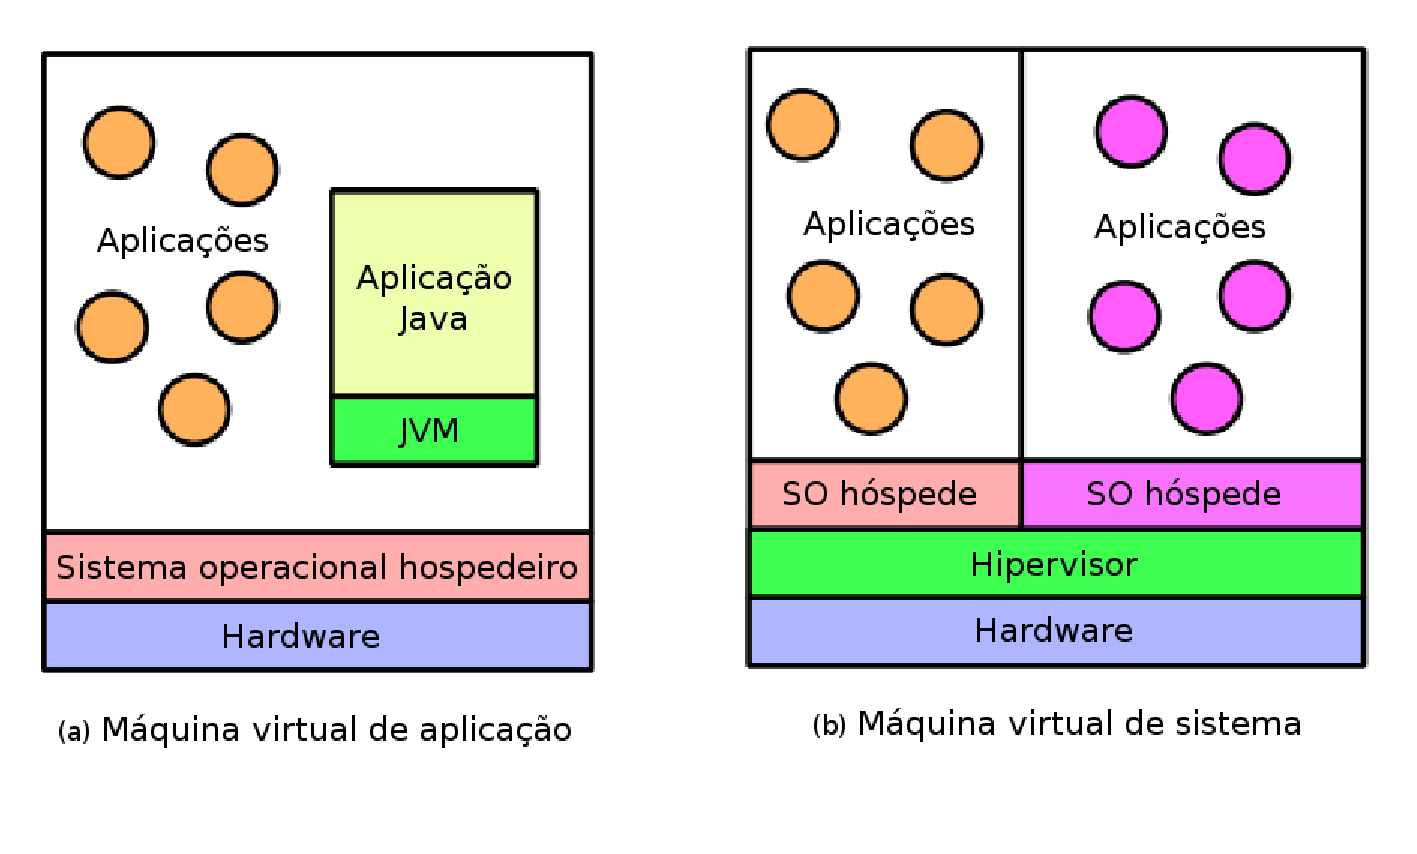
\includegraphics[width=320px]{img/vms_tipos.eps}
 \caption{Máquinas virtuais de aplicação e de sistema.}
 \label{fig:vms_tipos}
 Fonte: \citet{laureano2008}
\end{figure}

\section{Máquinas virtuais de aplicação}
\label{section:virtaplicacao}

As máquinas virtuais de aplicação, também chamadas de máquinas virtuais de processo, é geralmente conhecida por prover um ambiente
onde um sistema operacional suporte uma aplicação convidada, sendo que esta aplicação possui um conjunto de instruções ou de chamadas
do sistema diferentes do sistema hospedeiro.

Quando temos chamadas do sistema operacional ou instruções de máquina que são diferentes das oferecidas pela máquina real, será necessário
uma tradução dessas interfaces que será feita pela camada de virtualização. Exemplos dessa definição são:

\begin{itemize}
 \item Máquinas virtuais de linguagem de alto nível: este tipo de máquina virtual foi criado levando em consideração uma linguagem de 
 programação e seu compilador. O código compilado gera um código binário que não pode ser executado em nenhuma arquitetura real, mas pode
 ser executada em uma máquina virtual. Sendo assim para cada arquitetura ou sistema operacional deve existir uma máquina virtual que faça
 esse intermédio permitindo a execução de aplicações em sistemas operacionais diversos. Exemplos são: \textit{Microsoft Common Language 
 Infrastructure}, base do \textit{.Net} e a máquina virtual Java (\ac{JVM}) \cite{carissimi2008};
 \item Emulação no sistema operacional: ocorre quando as interfaces restringe-se às chamadas do sistema operacional, ou seja,
 é feito um mapeamento das chamadas utilizada pela aplicação com as chamadas do sistema operacional da máquina real. Este tipo de 
 virtualização de aplicação pode ser encontrado em ferramentas que emulam uma aplicação desenvolvida para uma plataforma em outra
 plataforma distinta. Como por exemplo o \textit{Wine}, que resumidamente permite executar aplicações \textit{Windows} em plataformas
 \textit{Unix}.
\end{itemize}

Na virtualização de aplicação também existem máquinas virtuais que utilizam as mesmas interfaces \ac{ISA} da máquina real,
com isso uma grande parte das instruções podem ser executadas diretamente, com exceção de instruções sensíveis, que serão devidamente
tratadas. Alguns tipos de máquinas virtuais de aplicação que utilizam as interfaces da máquina real são detalhadas abaixo:

\begin{itemize}
 \item Sistemas operacionais multi-tarefas: sistemas operacionais que suportam simultaneamente mais de um usuário também podem ser
 vistos como máquinas virtuais. Em um sistema multi-tarefa cada processo possui um ``processador virtual'' (devido a rápida troca de 
 contextos do processador real), uma ``memória virtual'' (memória alocada para o processo) e outros recursos que podem ser acessados
 através de chamadas de sistema;
 \item Tradutores dinâmicos: esses tradutores analisam e otimizam o código de máquina para torná-lo mais eficiente. Essa otimização 
 pode ser feita durante a carga do processo na memória ou durante a execução das instruções;
 \item Depuradores de memória: são sistemas de depuração de memória que detectam erros decorrentes do uso incorreto da memória.
 Um exemplo de depurador é o sistema \textit{Valgrind}, que faz a execução em uma máquina virtual.
\end{itemize}

\section{Máquinas virtuais de sistema}
\label{section:virtsistema}

Máquina virtual de sistema também pode ser chamada de hipervisor ou monitor (\ac{VMM}), que é uma camada de \textit{software} que possibilita
que um ou mais sistemas operacionais convidados executem independentemente sobre uma mesma máquina real. O hipervisor prove uma interface
\ac{ISA} virtual que pode ou não ser igual a interface real, e virtualiza outros componentes de \textit{hardware}, para então cada máquina
virtual convidada ter seus próprios recursos isolados.

Um ambiente de virtualização de sistema é composto basicamente por três componentes:
\begin{itemize}
 \item Sistema real: também pode ser chamado de hospedeiro, que é o \textit{hardware} onde o sistema de virtualização irá executar;
 \item Camada de virtualização: é conhecida como hipervisor ou também chamado de \ac{VMM} e tem como função criar interfaces virtuais a
 partir de interfaces físicas para a comunicação do sistema real com o sistema virtual;
 \item Sistema virtual: também conhecido como \textit{guest}, ou sistema convidado, que executa sobre o sistema real. Geralmente
 existem vários sistemas virtuais executando simultaneamente sobre o sistema real.
\end{itemize}

Virtualização de sistema utiliza abstração em sua arquitetura, por exemplo, ela transforma um disco físico em dois discos 
virtuais menores, sendo que esses discos virtuais são arquivos armazenados no disco físico. Sabendo que arquivos são uma abstração
em um disco físico, pode-se dizer que virtualização não é apenas uma camada de abstração do \textit{hardware}, ela faz a reprodução 
do \textit{hardware} \cite{smithenair2005}.

Pode-se classificar ambientes de máquinas virtuais de sistema de duas formas, pela arquitetura de virtualização 
(Seção \ref{section:virtarq}) ou pelo nível de virtualização (Seção \ref{section:virtniv}), ambos serão vistos nas próximas seções.

\subsection{Arquiteturas de virtualização}
\label{section:virtarq}

\begin{itemize}
 \item Hipervisores nativos: esse hipervisor executa diretamente sobre o \textit{hardware}, ou seja, sem um sistema operacional
 hospedeiro. O hipervisor nativo faz a multiplexação dos recursos do \textit{hardware} como memória, disco, entre outros,
 e diponibiliza esses recursos para as máquinas virtuais. Alguns exemplos que utilizam esse hipervisor são \textit{IBM 370}, 
 o \textit{Xen} e o \textit{VMware ESX Server};
 \item Hipervisores convidados: esse tipo de hipervisor executa sobre um sistema operacional hospedeiro, e utiliza os recursos 
 desse sistema para gerar recursos virtuais para as máquinas virtuais. Normalmente este tipo suporta apenas um sistema 
 operacional convidado para cada hipervisor. Exemplos de sistemas são o \textit{VirtualBox} e o \textit{QEmu}.
\end{itemize}

Sabendo essas definições pode-se concluir que hipervisor convidados são mais flexíveis que os nativos, pois podem ser implementados
em diversos sistemas operacionais e \textit{hardwares}. Já o hipervisor nativo possui melhor desempenho pois acessa o \textit{hardware}
diretamente.

\subsection{Níveis de virtualização}
\label{section:virtniv}

\begin{itemize}
 \item Virtualização de recursos: neste tipo de virtualização os recursos como memória e disco, além das instruções 
 privilegiadas (\textit{system \ac{ISA}}) são virtualizadas. Somente a interface \ac{ISA} de usuário é utilizada diretamente, 
 por isso o desempenho do sistema convidado é mais próximo a um sistema executando diretamente sobre um \textit{hardware}. O 
 \textit{VirtualBox} e o \textit{VirtualPC da Microsoft} são exemplos de virtualização de recursos;
 \item Virtualização completa: na virtualização completa todas interfaces são virtualizadas. Sendo assim o hipervisor fornece uma
 interface distinta ao sistema operacional convidado. Esse tipo de virtualização possui um eficiência menor, por outro lado ele
 permite executar sistemas operacionais em plataformas distintas a qual foram projetadas inicialmente. Por exemplo, o 
 \textit{MS Virtual PC for MAC}, que permite executar o sistema \textit{Windows} sobre plataforma de \textit{hardware} \textit{PowerPC}.
\end{itemize}

Tendo essas classificações, pode-se combiná-las para se obter quatro maneiras diferentes de implementar virtualização. Na Figura 
\ref{fig:vms_classificacao} tem-se essas combinações com seus respectivos exemplos.

\begin{figure}[vms_classificacao]
 \centering
 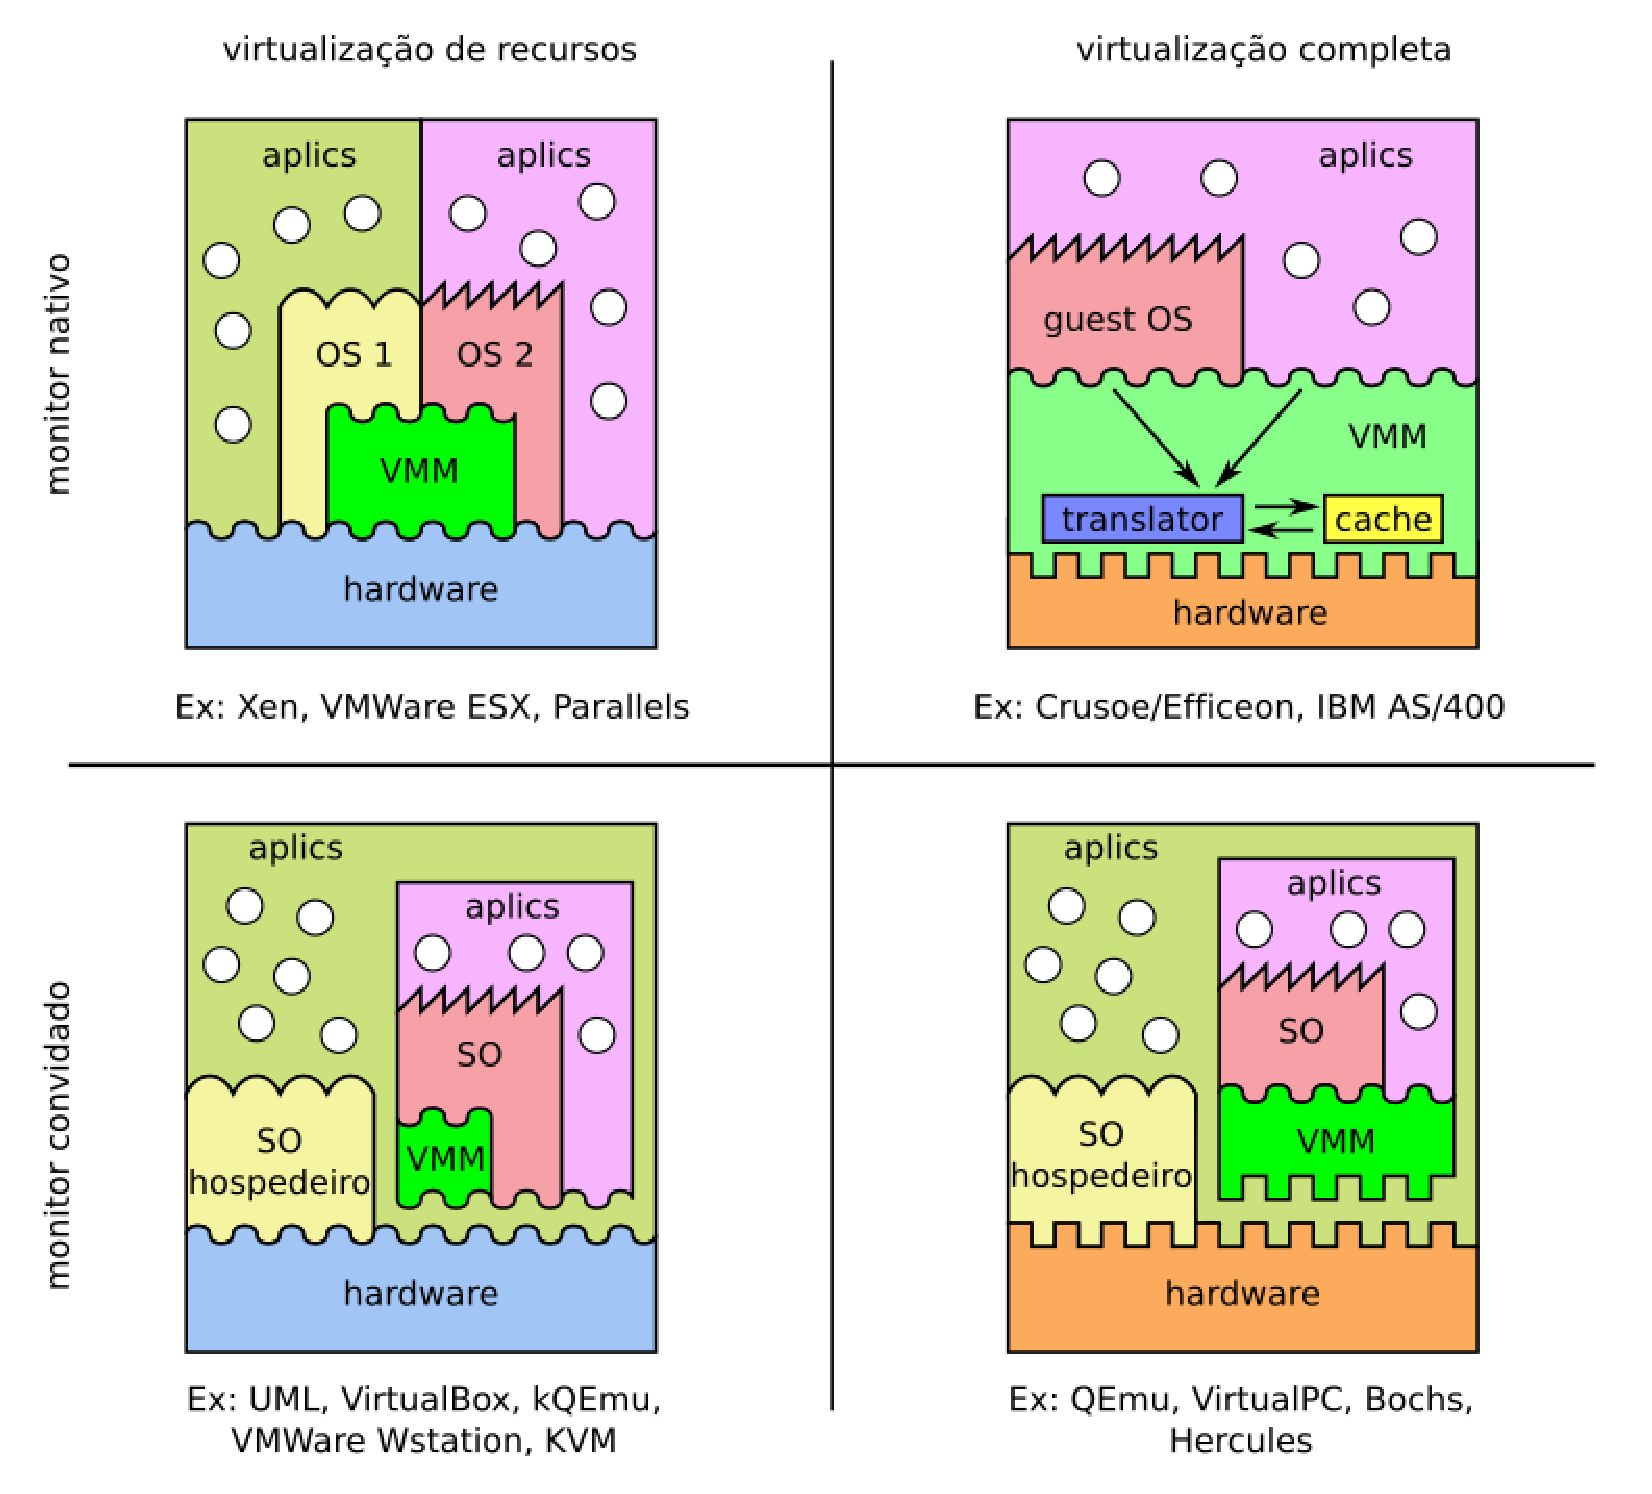
\includegraphics[width=400px]{img/vms_classificacao.eps}
 \caption{Classificação de máquinas virtuais de sistema.}
 \label{fig:vms_classificacao}
 Fonte: \citet{laureano2008}
\end{figure}

\subsection{Estratégias de virtualização}
\label{section:virtestrat}

Pode-se dividir máquinas virtuais de sistema em dois tipos de estratégias distintas, são elas:

\begin{itemize}
 \item Virtualização total: nesta estratégia todas as interfaces de acesso ao \textit{hardware} são virtualizadas. Desta forma
 possibilita-se que sistemas operacionais convidados executem como se estivessem diretamente sobre o \textit{hardware}. A grande
 vantagem dessa virtualização é a possibilidade de um sistema convidado executar normalmente sem precisar ser modificado. Porém
 existe uma redução significativa no desempenho devido ao hipervisor intermediar todas as chamadas e operações do sistema convidado.
 Exemplo de virtualização total é o \textit{QEmu};
 \item Paravirtualização: esta prove um melhor acoplamento entre o sistema operacional convidados e o hipervisor. Para isso o sistema
 convidado deve ser adaptado para o hipervisor no qual executará, ou seja, a interface de sistema (\textit{system ISA}) será acessada
 diretamente pelo sistema convidado, com isso haverá um melhor desempenho. Um exemplo de paravirtualização é o \textit{Xen}.
\end{itemize}

A paravirtualização possui um desempenho melhor comparado a virtualização total pois a primeira acessa alguns recursos diretamente, 
sendo que o hipervisor apenas monitora informando os limites do convidado. Por exemplo o gerenciamento da memória, na virtualização total
o hipervisor reserva um espaço para cada sistema convidado, que por sua vez acessa a memória como se fosse a memória de uma máquina física
iniciando seu endereçamento em zero. Sendo assim cada vez que o sistema convidado acessar a memória, o hipervisor precisará
converter os endereços do sistema convidado para endereços reais. Na paravirtualização o hipervisor informa ao sistema 
convidado a área de memória que ele pode utilizar, otimizando assim as operações.

A virtualização total obteve uma grande ganho de performance com a incorporação da virtualização aos processadores, através das 
tecnologias \ac{IVT} da \textit{Intel} e \ac{AMD-V} da \textit{AMD}. Elas possuem dois modos, um para execuções normais e para hipervisor, 
e outro específico para máquinas virtuais. 

\subsection{Um servidor por serviço}
\label{section:virtserv}

Em muitos casos empresas utilizam serviços distribuídos entre servidores físicos, como, por exemplo, servidores de e-mail, hospedagens e 
banco de dados, com isso existe uma ociosidade grande de recursos. Portanto uma das grandes vantagens da virtualização é um melhor 
aproveitamento destes recursos, alocando vários serviços em um único servidor físico e gerando um melhor aproveitamento do \textit{hardware} 
\cite{moreira2006}. Além disso, pode-se ter uma redução de custos com a administração e a manutenção dos servidores. Em um ambiente 
heterogênio pode-se também utilizar virtualização, pois ela permite a instalação de diversos sistemas operacionais em um único servidor.

Uma outra motivação para a utilização de virtualização consiste no custo da energia elétrica. A economia de energia pode ser obtida através 
da implantação de servidores mais robustos para substituir dezenas de servidores comuns. Outros fatores como refrigeração do ambiente e 
espaço físico utilizado também podem ser reduzidos com a implantação de virtualização de servidores, e consequentemente, reduzem os 
custos de energia.

A virtualização favorece a implementação do conceito um servidor por serviço, que consiste em ter um servidor para cada serviço.
Mas porque não colocar todos serviços em um único servidor? Muitas vezes com uma variedade de serviços é necessário diferentes 
sistemas operacionais, ou os serviços necessitam rodar nas mesmas portas, portanto isto se torna inviável. Outro fator relevante que 
também favorece a implementação de um servidor por serviço é, caso exista uma falha de segurança em apenas um serviço, essa 
vulnerabilidade poderá comprometer todos os outros serviços \cite{carissimi2008}.


%\begin{figure}[acoplamento_interfaces]
% \centering
% 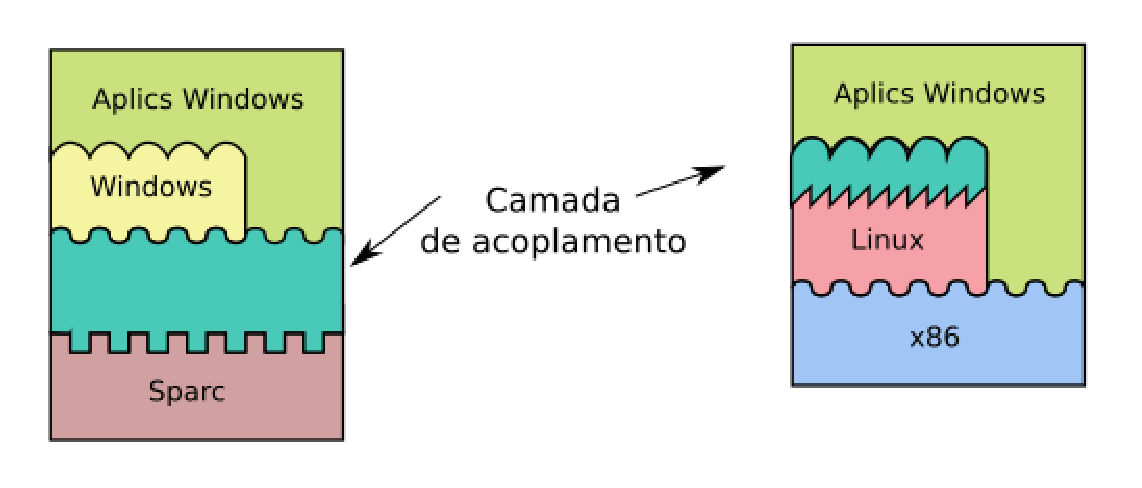
\includegraphics[height=140px]{img/acoplamento_interfaces.eps}
% \caption{Acoplamento entre interfaces distintas}
% \label{fig:acoplamento_interfaces}
% Fonte: \citet{laureano2008}
%\end{figure}
%Exemplo de camada de virtualização \ref{fig:acoplamento_interfaces} .... VER ONDE COLOCAR


\section{Emulação}
????


%Virtualizacao da teoria a solucoes:
%No entanto, essa abordagem trouxe como contra-partida a filosofia “um servidor
%por serviço”. Rapidamente, os responsáveis pelas áreas de TI se deram conta do
%problema (e custo) em gerenciar diferentes máquinas físicas, mesmo que tivessem o
%mesmo sistema operacional. Além disso, há problemas relacionados com consumo de
%energia elétrica, refrigeração, espaço físico, segurança física, etc. Nesse contexto, a
%virtualização surge como uma possibilidade de agregar os benefícios da componetização
%de sofware com a redução dos custos de manutenção de hardware e software. Assim, é
%possível manter a idéia de um “um servidor por serviço” sem ter um hardware
%específico.
%Essa abordagem é reforçada pela lei de Zipf [Adamic, 2008] que pode ser
%sintetizada da seguinte forma: a freqüência de um evento é proporcional a x −α , onde x é
%um ranking de comparação de um evento a outro. Alguns estudos [Breslau, Cao, Fan,
%Philips e Shenker, 2008] mostraram que a freqüência de acesso a servidores web e
%outros serviços Internet seguem uma distribuição Zipfian, o que, na prática, se traduz
%pelo fato de que a maioria dos acessos a serviços Internet é para uma minoria deles.
%Portanto, conclui-se que uma minoria de serviços está ativa enquanto a maioria está
%bloqueada a espera de requisições, o que, claramente, representa um desperdício de
%recursos. Para exemplificar, imagine, entre outros, o uso dos servidores de autenticação,
%DHCP, impressão, arquivos, e-mail, web e DNS em sua rede corporativa.

%Rejuvenescimento e migracao de vms:
%Com a arquitetura baseada em serviços, clientes podem utilizar serviços alocados em
%nuvem através dos web browsers. Unindo a computação em nuvem e a arquitetura baseada
%em serviços, aplicativos e demais recursos de TI podem ser oferecidos remotamente, como se
%estivessem localizados localmente. Vale a pena salientar que a arquitetura baseada em serviços
%permite monitorar em tempo real o uso dos recursos disponibilizados, colaborando assim para
%uma gerência mais eficiente a todo o sistema (LINTHICUM, 2009). Além disso, dependendo
%das interfaces definidas, pode-se ampliar consideravelmente o número de potenciais clientes.
%Recursos disponibilizados via navegador web, por exemplo, podem ser acessados tanto por
%computadores de mesa quanto por smartphones ou tablets.
%

%ver failover e failback em cluster?
